% !TEX root = ../document.tex

\chapter{系统面临的挑战}

目前根据前一章所提到的几个系统或者实验项目的结果来看,都提出了各自星基 ADS-B 系统在实践中面临的种种问题与挑战,主要包括以下几个方面。

\section{卫星星座规模与数据价值}

星基 ADS-B 主要是利用卫星上的接收机来接受 ADS-B 信号,进而实现对飞机位置的监视,卫星在接收到 ADS-B 信号之后,还需要将信号下行至地面网络,根据数据下行方式的不同,可以将星基 ADS-B 服务分为离线数据和在线数据两个方面。

通常而言,离线数据较容易实现,也通常被用于科学研究或者实验验证,它可以利用单颗卫星或者一小队卫星(3-6颗)在低地球轨道上接收 ADS-B 数据,然后将数据存储到自身携带的存储设备中,在卫星经过一个或者多个地面站时,数据将通过下行链路传递至地面站,这样的数据是有延迟的,通常会有大规模的延迟,不能实现实时监视,这种数据通常有两种意义,一是用于对技术进行验证或者研究数据质量等科学研究性质的目的;二是如果让这种数据发挥实用价值的话,如果某架飞机在洋区失踪了,如果在该飞机失踪时刻恰巧该卫星位于失踪飞机上方信号可接收范围内,这种数据可以提供飞机失踪前最后的位置报告。

展开来谈,低轨卫星的飞行速度非常快,90 分钟左右即可环绕地球一圈,单颗卫星在经过某架飞机上方时,只能接受到某架飞机极短的一段位置报告,如图\ref{fig:AOS-south_china}所示,是 AOS 实验项目中接收到的中国丽江机场某架飞机的航迹,在卫星飞过的过程中,仅接收到了短短一小段飞机的航迹,无法实现对某架飞机的连续跟踪,所以说单颗卫星的离线数据其应用价值不大。

\begin{figure}[!htb]
\centering
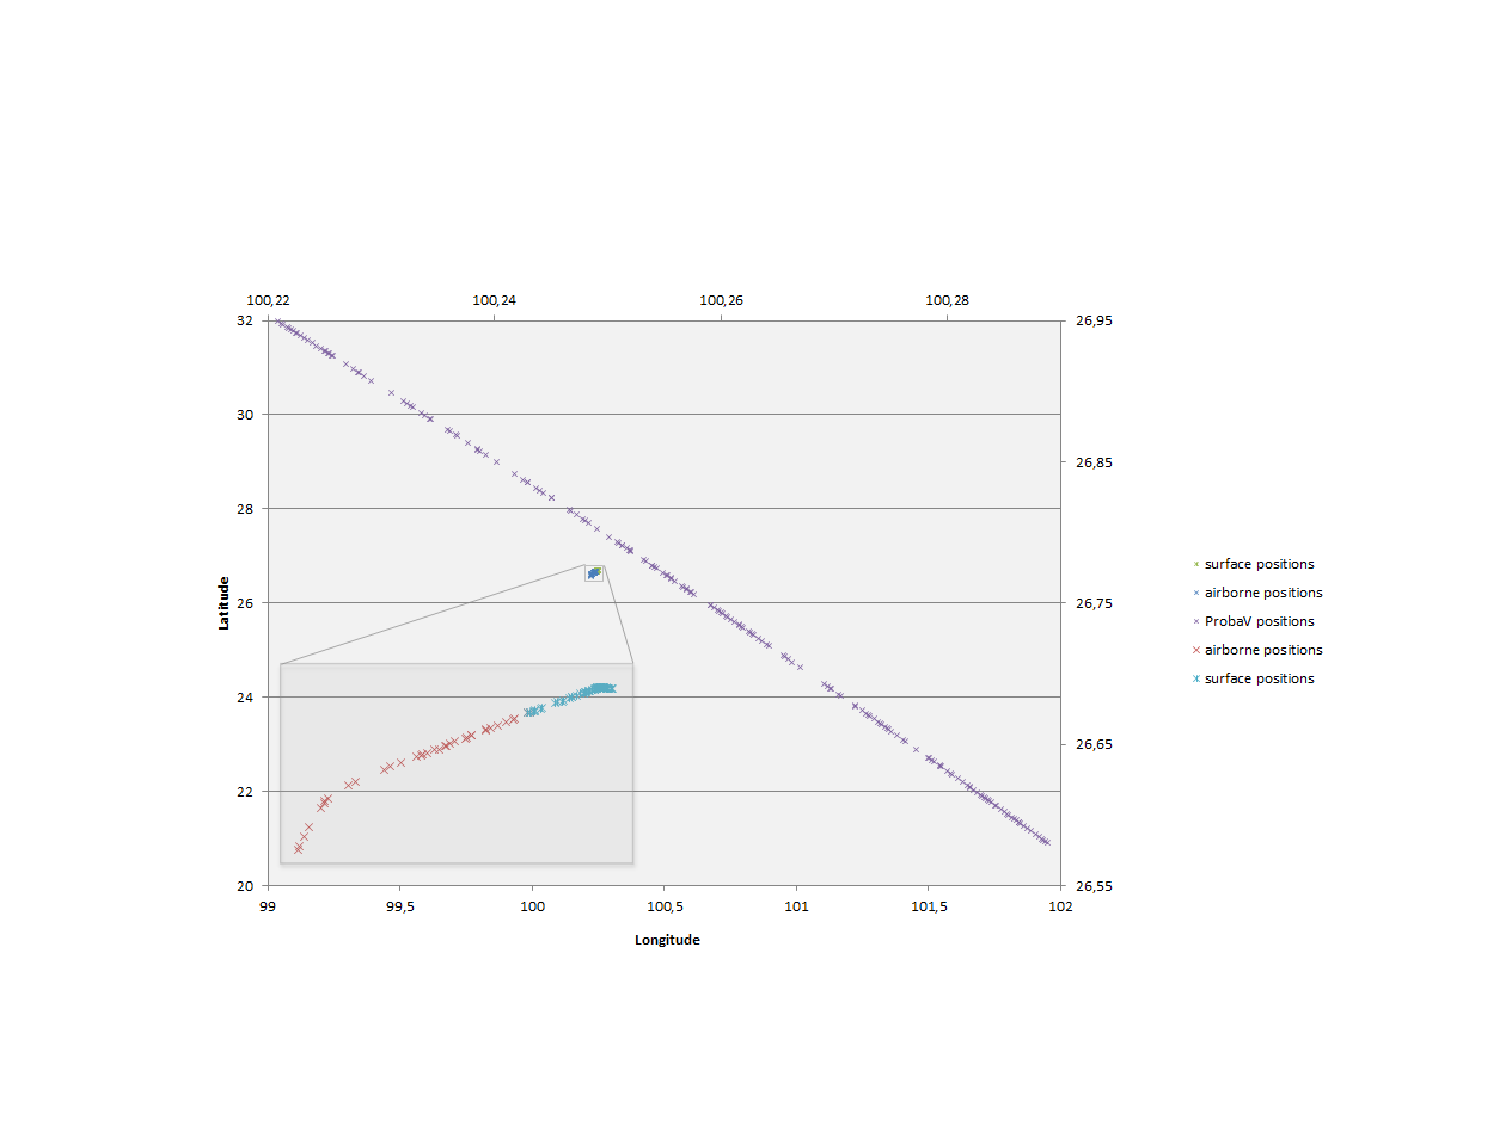
\includegraphics[width=13cm]{pic/AOS-south_china.pdf}
\caption{AOS 项目中接收到的中国丽江机场附近某架飞机的航迹\protect\footnotemark}
\label{fig:AOS-south_china}
\end{figure}

\footnotetext{图片来源:参考文献\cite{e2ppt}}

若想真正将该系统运用到实际中来,必须通过在线数据,从而必须实现卫星星座组网(40-70颗),采用卫星星座覆盖整个地球,才能够在同一时刻接收到全球飞机的 ADS-B 信号并实现对某一架飞机的连续跟踪,当一颗卫星超过某架飞机的信号接收范围时,另一颗卫星又处于该架飞机的信号接受范围内,可以继续接收该信号,但是这对数据处理提出了要求,要求数据处理算法能够无缝接洽两颗或多颗卫星上的同一飞机信号。通过卫星网络的数据下行也有多种方式,比如携带 ADS-B 接收器的卫星可以通过卫星间的网络将数据传输至地球同步数据中继卫星,数据中继卫星再近乎实时地连接到地面 ATM 设施。或者直接通过星基 ADS-B 卫星之间的通信网络将数据下传至固定的地面站,这即是在线数据传输。

地面站的数量也决定在线数据的延迟时间,这一点可以通过 Aireon 的铱星网络和 ALAS 的 Globalstar 看出区别,铱星网络地面站仅建在美国,但是依托其星座卫星数量多,并且可以实现星间通信,铱星网络可以通过星间通信将全球所有卫星采集的数据实时传输到位于美国上空的卫星,再通过位于美国上空的卫星将数据下传至地面站,最后通过地面网络发送至全球各地的用户。Globalstar 则采用了不同的思路,Globalstar 的星座数量不如铱星庞大,但是其在全球各地建立了多个地面关口站,大约有 33 个地面关口站,用于接收 24 颗 Globalstar 第二代卫星的数据,这样,所有卫星采集的数据都能不需通过星间链路而直接下传至地面,其数据延迟会大大减少。

建设卫星网络和多个地面站需要投入大量的资金。

\section{信号强度}

根据 DLR 的 AOS 实验项目,在信号强度上,该实验项目的结果提出了如下几个需要克服的问题。

\begin{enumerate}
    \item \textbf{由于信号相关性差,1090MHz S 模式格式不适用于接收弱信号(<-90dBm)}

    DLR 的 AOS 实验项目的卫星上的 FPGA 配备了一个 32 位嵌入式处理器来处理星载接口。通过 RS-422 UARTs 以 115kbps 的波特率与航天器通信并指挥接收机。接收机的输入灵敏度取决于传入消息的频率条件,最小触发电平约为 -96dBm。

    必须注意 LEO 中的有效载荷正在寻找非常弱的 Mode-S 信号。一般来说,在 -90dBm 以下的典型的飞机应答器应用还没有开发出来,而且相关性能很差。在这种创新的方法中,一种附加的信号处理算法也利用了发射信号的相位信息。该技术将在任务运行时进行测试和改进,因为接收器 FPGA 配置和处理器固件可以从地面更改。这个特性已经成功地测试过了。

    由于卫星上的限制,在轨道上没有对解码后的 S 模式电报位进行进一步的预处理。相反,所有的原始电报数据都向下连接到地面进行解码和分析。这允许最大的灵活性,因为系统不限于 DF17。\upcite{e2}


    \item \textbf{飞机与 LEO 卫星之间的距离约为 800 公里(444 海里)}

    1090ES ADS-B 的“正常”覆盖范围为:空中到空中为 50NM,空中到陆地为 150NM。

    在空间接收 ADS-B 报文最重要的方面是卫星上 1090MHz ES 信号的接收条件。接收卫星在大约 820 公里的高度,而发射信号的飞机大约在 0 至 12 公里的高度。与最大射程 300 公里的地面 ADS-B 监视相比,在 820 公里高度运行的 LEO 卫星与飞行器之间的信号路径要长得多,导致 ADS-B 接收机的信号电平较低。因此,S模式信号必须在噪声水平上通过相关处理进行检测。

    \item \textbf{关于信号的其他因素}

    另外如下几条因素也可能导致 ADS-B 信号丢失。

    \begin{itemize}
        \item 由于卫星天线垂直辐射模式和飞机天线垂直辐射模式的形状造成的射频信号损失

        \item 当多个到达卫星机载 ADS-B 天线的消息同时重叠,从而无法被 ADS-B 接收机解码

        \item 如上一节所说,卫星的速度约为 27000 公里/小时,因此每架探测到的飞机的观测时间有限,最多约 3 分钟

        \item 此外,由于将卫星上的 ADS-B 接收器作为有效载荷加以集成,基于卫星的监测的轨道内试验演示受到进一步的限制:考虑到卫星上其他的有效载荷,卫星必须调整姿态作出有利于其他有效载荷进行观测的姿态,这会影响 ADS-B 信号的接收

        \item 天线安装位置不是直接为基于 1090ES 的空间接收优化,而是为了不干扰主卫星任务和其他承载有效载荷而做出的妥协

    \end{itemize}

\end{enumerate}

综上所述,要优化 ADS-B 信号的接收,卫星必须为该任务进行专门的设计。


\section{调制方案}

DLR 的 AOS 实验项目的实验结果声称脉冲位置调制(PPM)不适合对噪声水平附近的信号进行解码,但并未给出原因。


\section{静锥区}

上一章提及的多个项目都提到了静锥区对信号接收的影响。

飞机装有两个 ATC 天线,一个在机身顶部,一个在机身底部,它们交替发射。由于几何因素限制,卫星将接收来自顶部天线的信号。顶部天线典型的垂直天线辐射模式如图\ref{fig:antenna_of_plane-1}所示。

\begin{figure}[!htb]
\centering
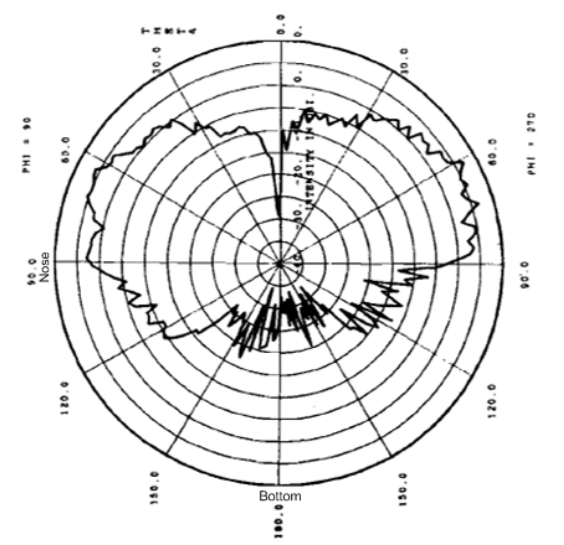
\includegraphics[width=10cm]{pic/antenna_of_plane.png}
\caption{顶部安装的 L 波段天线的垂直天线辐射图\protect\footnotemark}
\label{fig:antenna_of_plane-1}
\end{figure}

\footnotetext{图片来源:参考文献\cite{e2ppt}}

该形状为环形,中心凹处为 0 度,即朝向天顶的方向,于是在飞行器垂直上方形成所谓的“静锥区”,这个静锥区是发射天线中的常见问题,一般对于雷达来说,由于其仰角的限制,同样存在所谓的颈椎区,即雷达正上方区域是辐射无法到达的区域。

因此,在卫星上,或多或少位于卫星正下方的飞行器可能不会被探测到。应该指出,根据天线的安装位置和机身的几何形状,不同飞机类型的辐射模式有很大的不同。所以对一些飞机来说,中心凹处更宽,凸起处更浅。

而接下来再看卫星上的 ADS-B 信号接收器的天线辐射图,如图\ref{fig:ADS-B_Auto4-1}所示。

\begin{figure}[!htb]
\centering
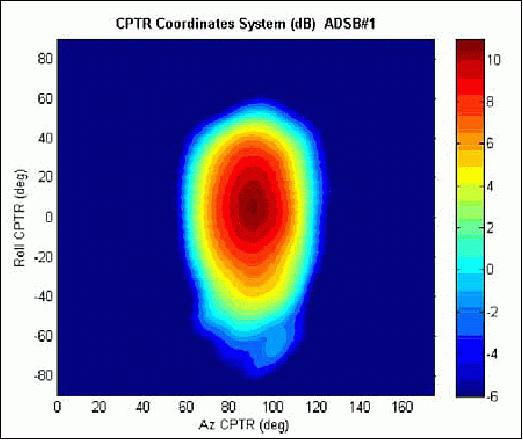
\includegraphics[width=10cm]{pic/ADS-B_Auto4.jpeg}
\caption{Proba-V 卫星天线辐射图\protect\footnotemark}
\label{fig:ADS-B_Auto4-1}
\end{figure}

\footnotetext{图片来源:参考文献\cite{e2ppt}}

DLR 的 AOS 实验得到了卫星天线覆盖区中不同区域接收到的 ADS-B 报文数量分布的足迹,如图\ref{fig:ADS-B_Auto5-1}所示,该图显示了 2014 年 5 月收到的所有位置消息的足迹。值得注意的是两个峰值,一个在卫星运动方向前方,峰值较低,另一个在卫星运动方向后方,峰值较高。这个谱的分布是不对称的,这由许多原因引起,比如卫星上的贴片天线的安装位置不对称、安装在卫星下侧的其他设备和在下表面的前边缘上突出的太阳能电池板。

\begin{figure}[!htb]
\centering
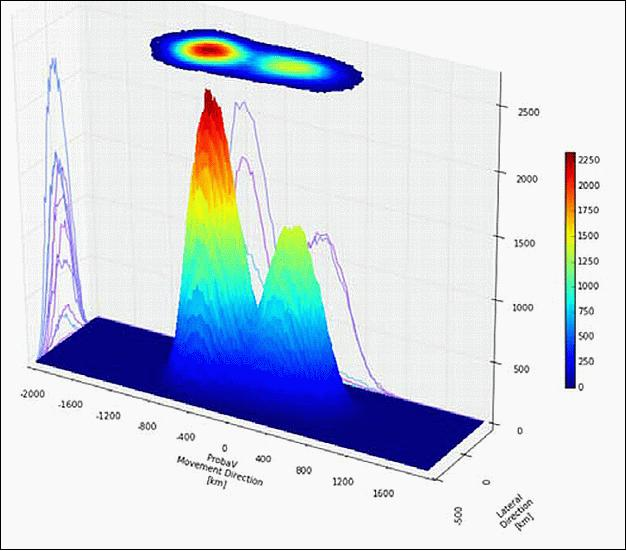
\includegraphics[width=10cm]{pic/ADS-B_Auto5.jpeg}
\caption{所有接收到的位置信息在天线覆盖区中的分布足迹\protect\footnotemark}
\label{fig:ADS-B_Auto5-1}
\end{figure}

\footnotetext{图片来源:参考文献\cite{e2ppt}}

从足迹的形状,即图\ref{fig:ADS-B_Auto5-1}可以看出,这两种“互补”的辐射模式并不相互补偿,导致 ADS-B 信号接收在足迹中间形成一个清晰的凹槽,这是由飞机天线的“静锥区”造成的。

在上一章中,同样提及了 Aireon 的星基 ADS-B 项目中对于静锥区的考虑。该项目中提及,航空电子设备标准确定了功率输出为 125 瓦、250 瓦和 500 瓦的机载发射机的等级,当全球的飞机上的发射器都以 250W 的功率工作时,其 L 波段天线上方的静锥区非常小,这影响可以忽略不计,这时 Aireon 的卫星网可以实现对全球飞机的全部覆盖,即收到所有飞机的信号,这时的模式图如图\ref{fig:CPWG16_PPT09_Satellite_Based_ADSB_December2013_1-1}所示。而当全球所有飞机都以 125W 的功率工作时,这时位于卫星正下方的飞机的静锥区的影响不可以不考虑,会产生监控盲区,也就是位于卫星正下方的飞机是看不到的,这时卫星监控范围如图\ref{fig:CPWG16_PPT09_Satellite_Based_ADSB_December2013-1}所示。

\begin{figure}[!htb]
\centering
\begin{minipage}[t]{0.48\textwidth}
\centering
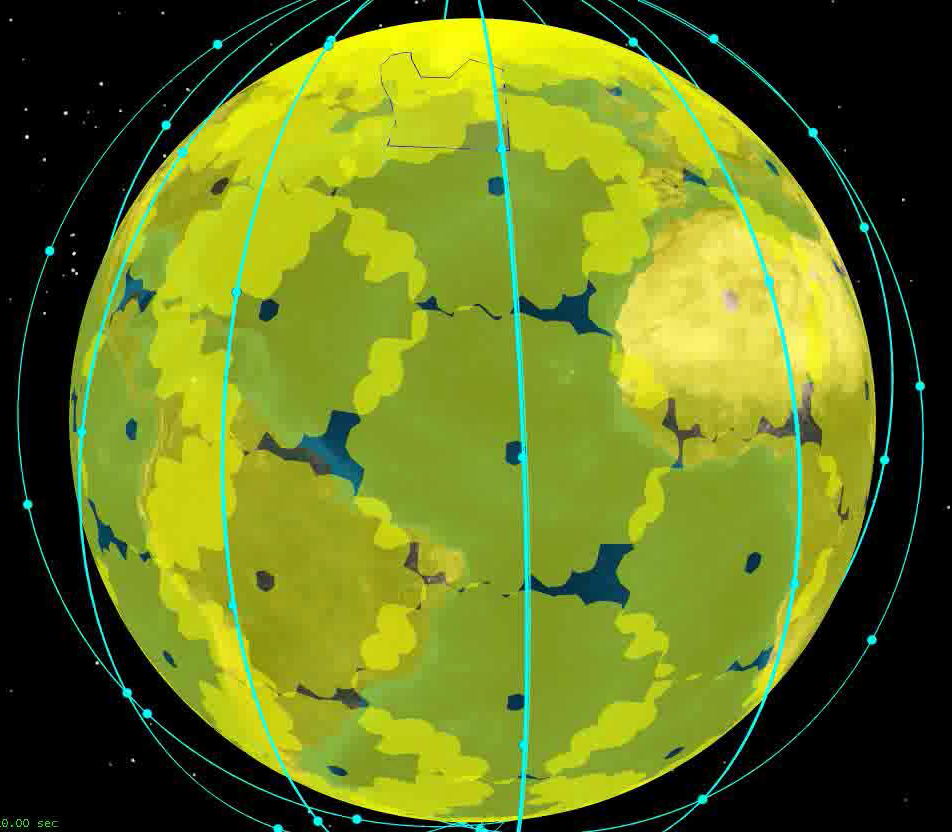
\includegraphics[height=6cm]{pic/CPWG16_PPT09_Satellite_Based_ADSB_December2013.png}
\caption{125W 功率下的全球覆盖范围\protect\footnotemark}
\label{fig:CPWG16_PPT09_Satellite_Based_ADSB_December2013-1}\footnotetext{图片来源:参考文献\cite{e13}}
\end{minipage}
\begin{minipage}[t]{0.48\textwidth}
\centering
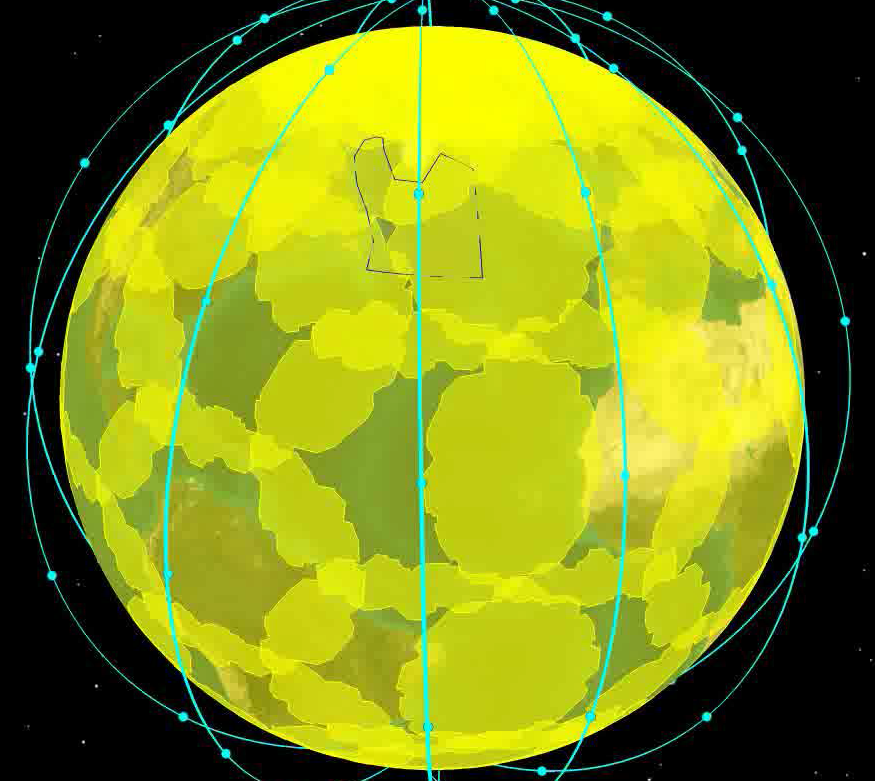
\includegraphics[height=6cm]{pic/CPWG16_PPT09_Satellite_Based_ADSB_December2013_1.png
}
\caption{250W 功率下的全球覆盖范围\protect\footnotemark}
\label{fig:CPWG16_PPT09_Satellite_Based_ADSB_December2013_1-1}\footnotetext{图片来源:参考文献\cite{e13}}
\end{minipage}
\end{figure}

这个静锥区可以用图\ref{fig:cone_of_silence}解释,125W 应答器会造成这种监视空档,Aireon 对空档的说明如下:

\begin{itemize}
    \item 空档相对较短,对于 125W 的飞机来说,最多 35 秒
    \item 目前这种由静锥区引起的间隙导致 1 或 2 次更新暂时丢失,更新速度为 15 秒,相当于雷达滑行
    \item 对于海洋航班,即使有锥形静音,Aireon 15 秒更新的时间百分比也远远超过 95\%
\end{itemize}

\begin{figure}[!htb]
\centering
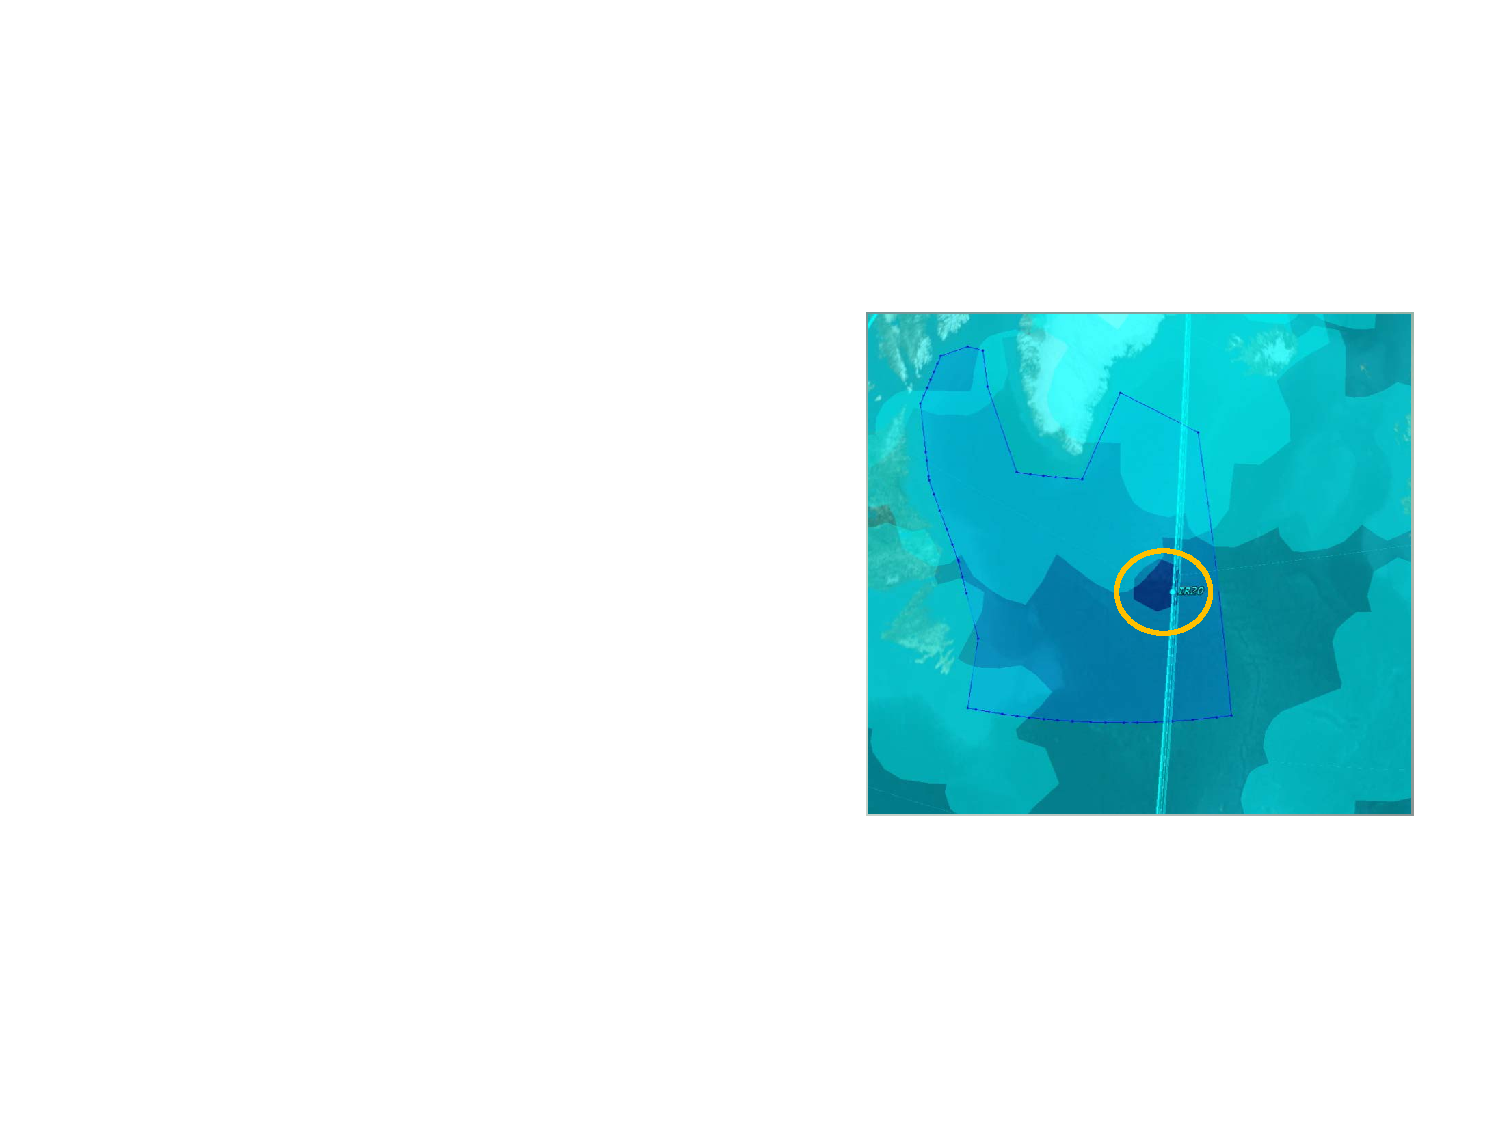
\includegraphics[width=8cm]{pic/cone_of_silence.pdf}
\caption{静锥区的影响\protect\footnotemark}
\label{fig:cone_of_silence}
\end{figure}

\footnotetext{图片来源:参考文献\cite{e13}}

\section{报文冲突}

丹麦的 GATOSS 实验项目提供的实验结果中提示了报文冲突的问题,卫星将看到大面积的 ADS-B 信号干扰拥挤的空域。

\begin{itemize}
    \item 在拥挤的空域(如中欧上空),预计操作不可行,但在覆盖海洋区域方面,预计有足够的性能

    \item GATOSS 任务将准确描述哪里有可能提供操作服务,哪里没有
\end{itemize}

如图所示,在航班拥挤的空域,接收到的 S 模式报文在解码时存在困难,而在洋区接收到的 ADS-B 报文,由于报文数量没有如此拥挤,故报文的提取与检测相对简单。

\begin{figure}[!htb]
\centering
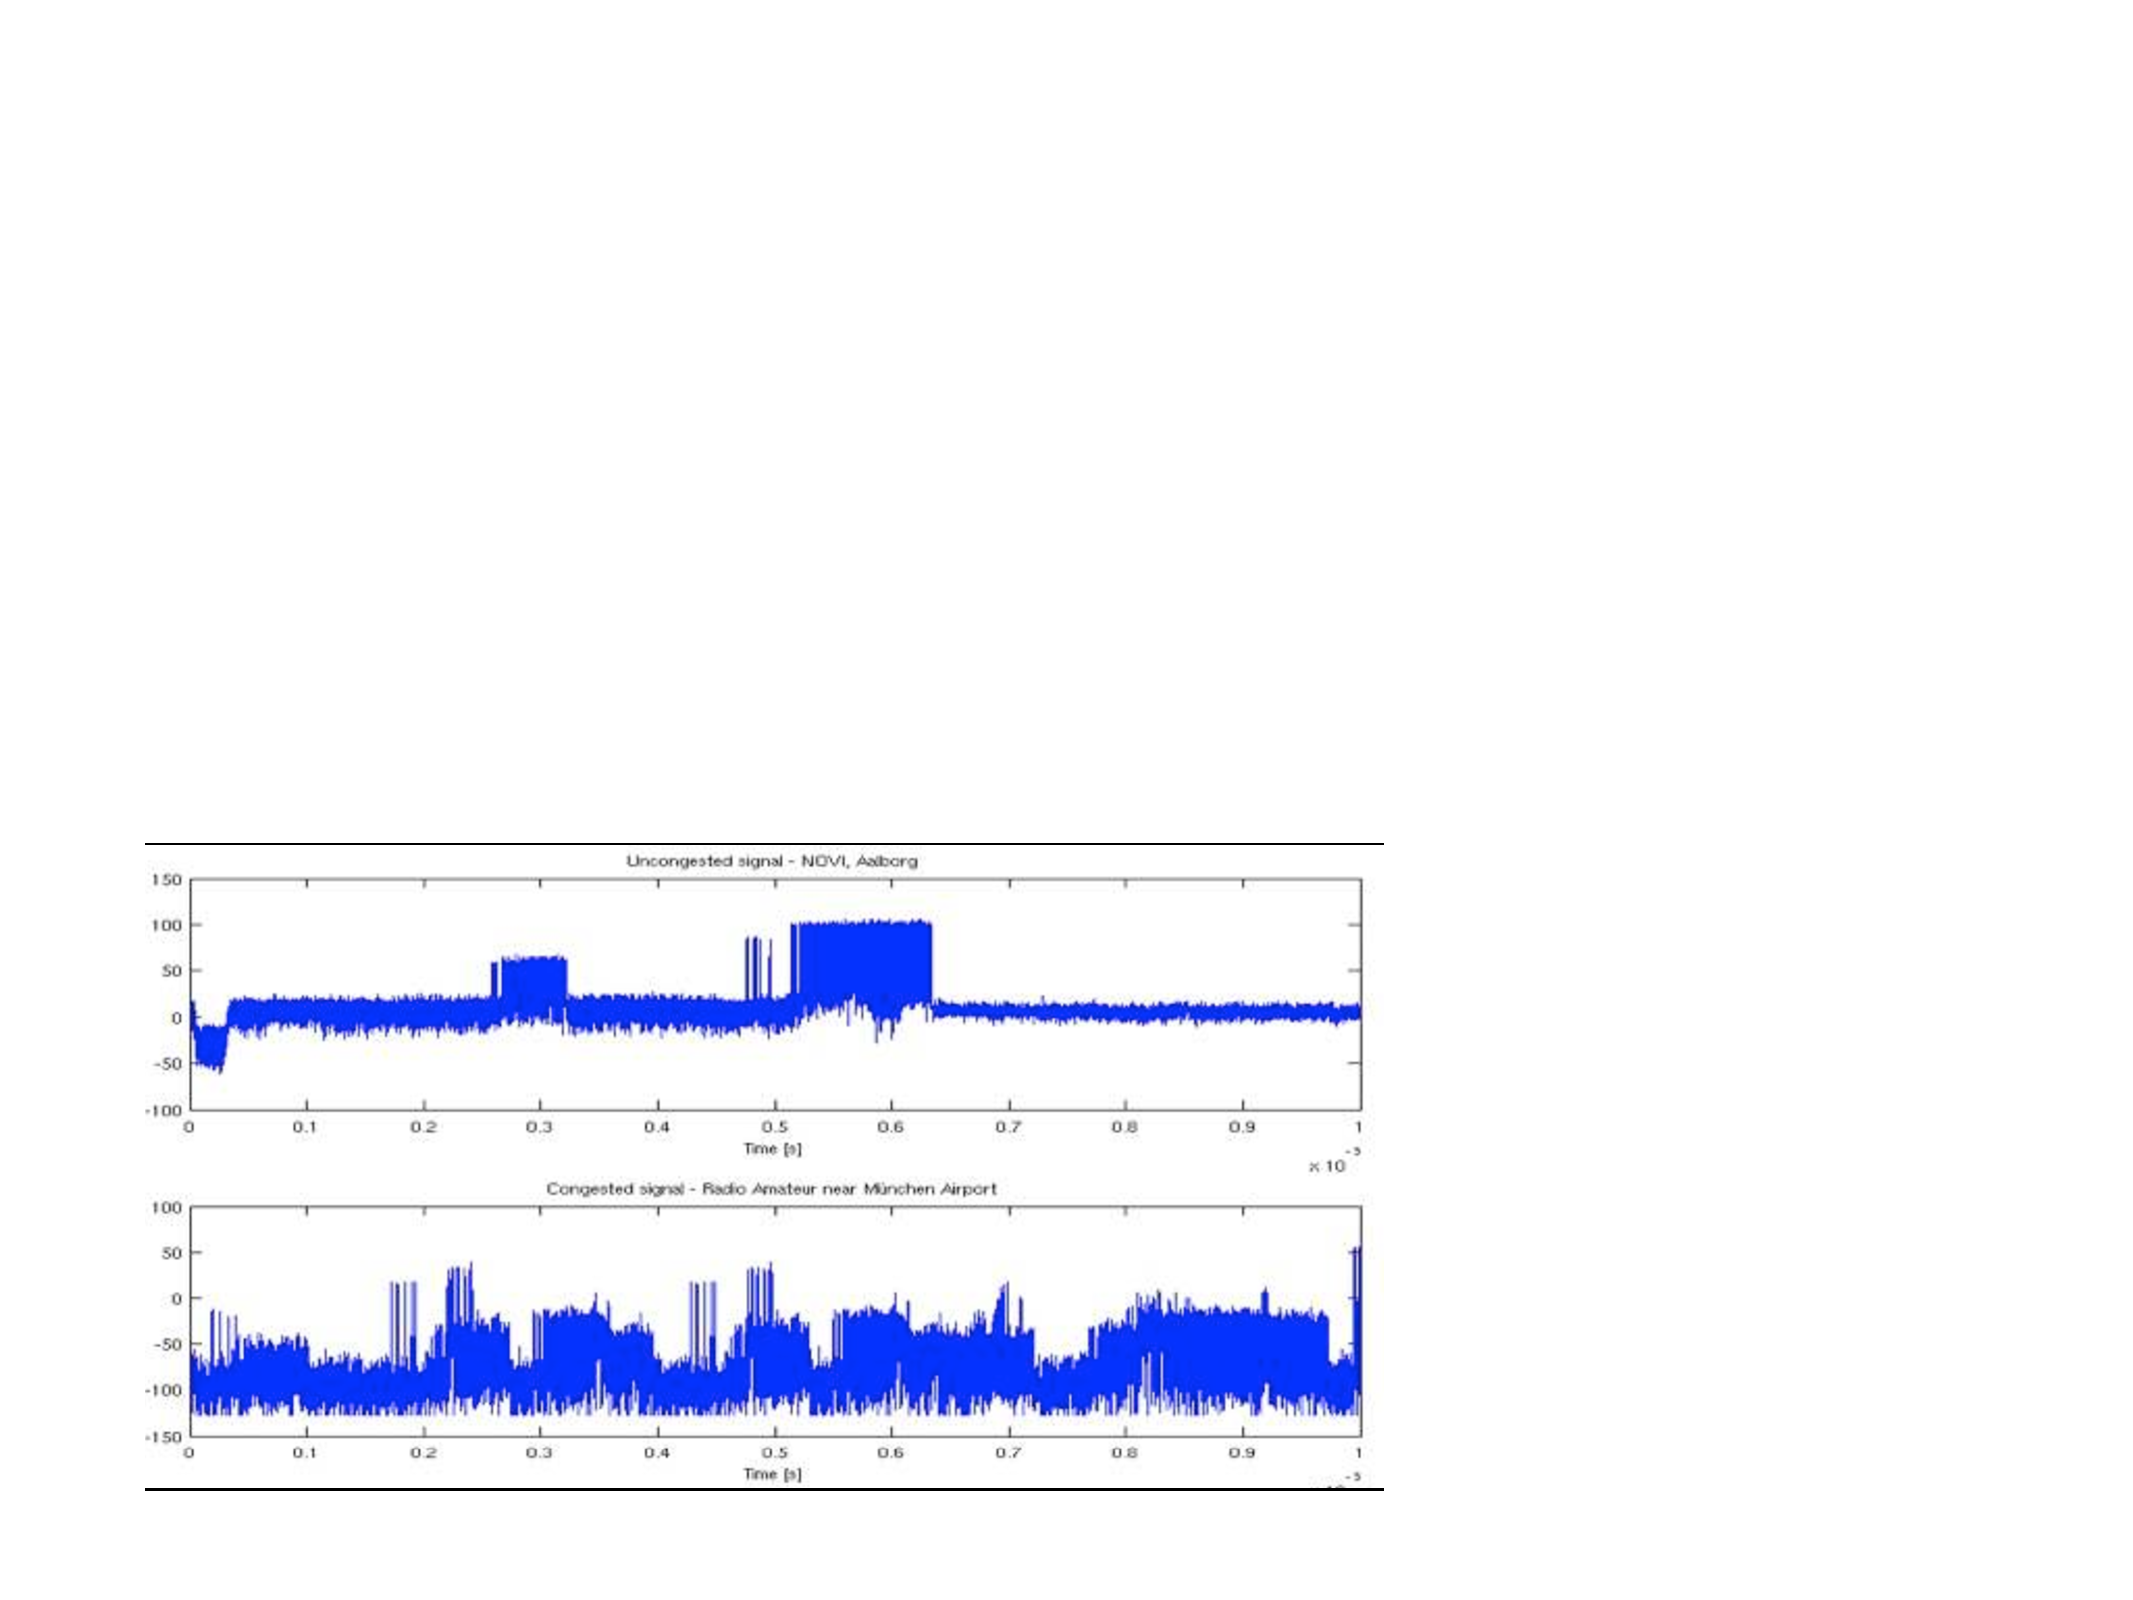
\includegraphics[width=12cm]{pic/data_collision.pdf}
\caption{报文冲突\protect\footnotemark}
\label{fig:data_collision}
\end{figure}

\footnotetext{图片来源:参考文献\cite{e17}}

\section{其他的考虑}

目前星基 ADS-B 技术中仍然存在其他一些问题,但基本都是上述主要因素衍生的。其他的问题集中在数据质量、监视性能、数据通信等问题。

对于星基 ADS-B 信号数据质量的研究,可以参看文献\cite{z2},对于星基 ADS-B 监视性能的研究,可以参看文献\cite{z4,z5,z6,e18}。

另外,ADS-B可以利用甚高频(VHF)自组织数据链实现,但是其监视范围局限在视距以内, 因此需要引入卫星数据链以实现超视距监视,从而形成综合这两种数据链的组合监视系统。同时, 为了适应网络拓扑的快速变化,并高效利用网络资源传输信息,必须引入分群技术\upcite{z3}。文献\cite{z3}研究了空基与星基组合监视系统的实现问题,并研究了系统中的 ADS-B 分群算法。并提出一种综合最大连通度和非确定性准则的分群算法,用以解决分群技术组网收敛速度和网络稳定性之间的矛盾。

另外还存在对于星基 ADS-B 链路的预算的研究,参看文献\cite{z9}。






